\subsection{GPU Hough}

The Hough algorithm operates iterating over all pixels of an image.
As such, a new approach was developed, where this loop is replaced by a parallel GPU kernel call.

\subsubsection{Algorithm}

The general algorithm is the same as presented in~\ref{sec:locate:hough}, with all steps executed in GPU.
In particular:
\begin{itemize}
	\itemsep 0em
	\item Step 1 is performed by a kernel, with synchronization after it;
	\item Step 2 is executed by a separate kernel, with synchronization after;
	\item Steps 3 and 4 are run by a unique kernel, that executes non-max suppression on its own pixel, and if it not suppressed, uses atomic methods to add the pixel as coordinate center.
\end{itemize}
On top of the pixels of each frame, also the frames themselves were processed in parallel.

\subsubsection{Evaluation}

The performance of this approach is worse than the CPU Hough transform, both in quality and speed: the algorithm only identifies about 65\% of the bubbles (as visible in figure~\ref{fig:locate:gpu-hough}), running at 17 FPS.

\begin{figure}
	\centerline{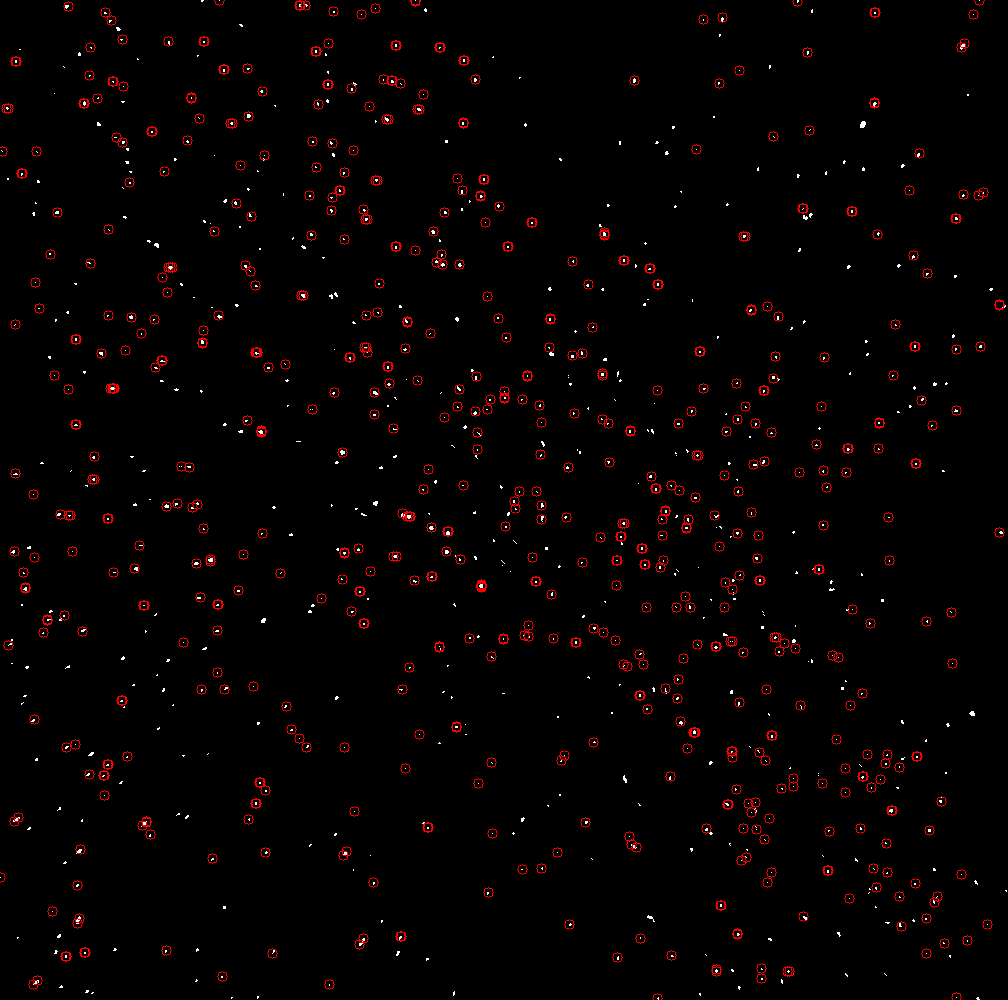
\includegraphics[width=\locateimgsize]{images/locate/my-hough-transform.png}}
	\caption{\centering GPU Hough's result}
	\label{fig:locate:gpu-hough}
\end{figure}
